%=============================================================================
% MIA 5100 — Snap-to-Sell — Final Report (IEEE conference format)
% Build:  pdflatex final_report -> bibtex final_report -> pdflatex x2
% Needs a TeX distro providing IEEEtran.cls and IEEEtran.bst (TeX Live / MacTeX).
% Target length: 5 pages. Keep prose justified; do not paste template guidance back in.
%=============================================================================
\documentclass[conference]{IEEEtran}
\IEEEoverridecommandlockouts
\usepackage{cite}
\usepackage{amsmath,amssymb,amsfonts}
\usepackage{graphicx}
\usepackage{booktabs}
\usepackage{textcomp}
\usepackage{xcolor}
\usepackage[hidelinks]{hyperref}
\graphicspath{{figures/}}

\begin{document}

\title{Snap-to-Sell: An Open-Source Pipeline for Turning a Corner-Store Product Photo into a
Priced, Image-Upgraded Listing}

\author{
\IEEEauthorblockN{Ikenna Okonkwo\IEEEauthorrefmark{1}, [Member 2], [Member 3], [Member 4], [Member 5]}
\IEEEauthorblockA{School of [Program], University of Ottawa\\
MIA 5100 --- Machine Learning\\
\{iokon081, \dots\}@uottawa.ca}
}

\maketitle

%------------------------------------------------------------------------------
\begin{abstract}
% TODO WS5 (write last, ~150-200 words): objectives, approach, key findings.
Independent corner stores struggle to digitise inventory for online sale because creating a
catalogue entry per product is slow and manual. We present Snap-to-Sell, an open-source pipeline
that turns a single phone photo of a packaged product into a publishable listing: it recognises
the item with a vision--language model fused with packaging OCR, retrieves a canonical name,
price, and licensed product image from Open Food Facts and Open Prices, generates grounded
listing copy, replaces the shelf photo with a verified higher-resolution catalogue image, and
applies responsible-AI guardrails (age-restricted-item flagging, hallucination and
low-confidence routing) before human review. We evaluate the pipeline on a hand-labelled set of
approximately fifty corner-store products across [N] categories, measuring identification
accuracy, price error, listing quality, age-restriction recall, and the rate of incorrect image
swaps. % TODO: one sentence of headline results.
\end{abstract}

\begin{IEEEkeywords}
retail product recognition, vision--language models, e-commerce, listing generation, price
estimation, responsible AI
\end{IEEEkeywords}

%------------------------------------------------------------------------------
\section{Introduction and Background}
% TODO WS5: the field (packaged-goods e-commerce onboarding), why it matters now, key terms
% (VLM, OCR, retrieval grounding), scope and objectives. Draw from ../execution_plan.md and
% ../literature_review.md. 2-3 short paragraphs.

%------------------------------------------------------------------------------
\section{Problem Statement and Motivation}
% TODO WS5: define the core problem — can a single photo of a packaged product be turned,
% accurately enough to be useful, into a publishable, correctly priced listing? Why it is
% significant for small retailers, and why identity+price+non-misleading copy is the hard part.

%------------------------------------------------------------------------------
\section{Related Work}
% Prose drafted in ../related_work_draft.md — condense to fit. Citations resolve from
% references.bib (verify the entries tagged TODO before submission).
Automatically turning a product photograph into a priced listing draws on four established
threads: listing-text generation, fine-grained product recognition, price estimation, and
product image retrieval. Recent listing-generation work favours frozen foundation models: ModICT
generates descriptions from an image and keywords using a frozen language model with in-context
references, and names the failure we guard against---generic, inaccurate copy for same-category
products~\cite{li2024modict,ijsr2024listing}. Fine-grained recognition of packaged goods is well
supported by large datasets such as RP2K and the smartphone-captured CAPG-GP
collection~\cite{peng2020rp2k,geng2018oneshot}, and fusing the product image with packaging OCR
outperforms image-only recognition, especially with few samples~\cite{grocery2023ocr}. Price
estimation has moved from image-only regression~\cite{chen2018priceright,secondhand2020deep}
toward retrieval-grounded, confidence-aware generation~\cite{llp2025}. Finally, the image-upgrade
step rests on product visual search and same-product verification~\cite{sir2020,shin2022eclip},
which also supply restricted-item detection reusable for our age-restriction guardrail.
% TODO WS5: add the comparison table from ../literature_review.md as Table~\ref{tab:related}.

%------------------------------------------------------------------------------
\section{Methodology}
% TODO WS5: end-to-end workflow overview; reference Fig.~\ref{fig:arch} and Fig.~\ref{fig:dataflow}.
Snap-to-Sell is a staged pipeline with a human-in-the-loop checkpoint before publication, shown
in Fig.~\ref{fig:arch}. The data artifacts exchanged between stages are shown in
Fig.~\ref{fig:dataflow}.

\begin{figure}[t]
\centerline{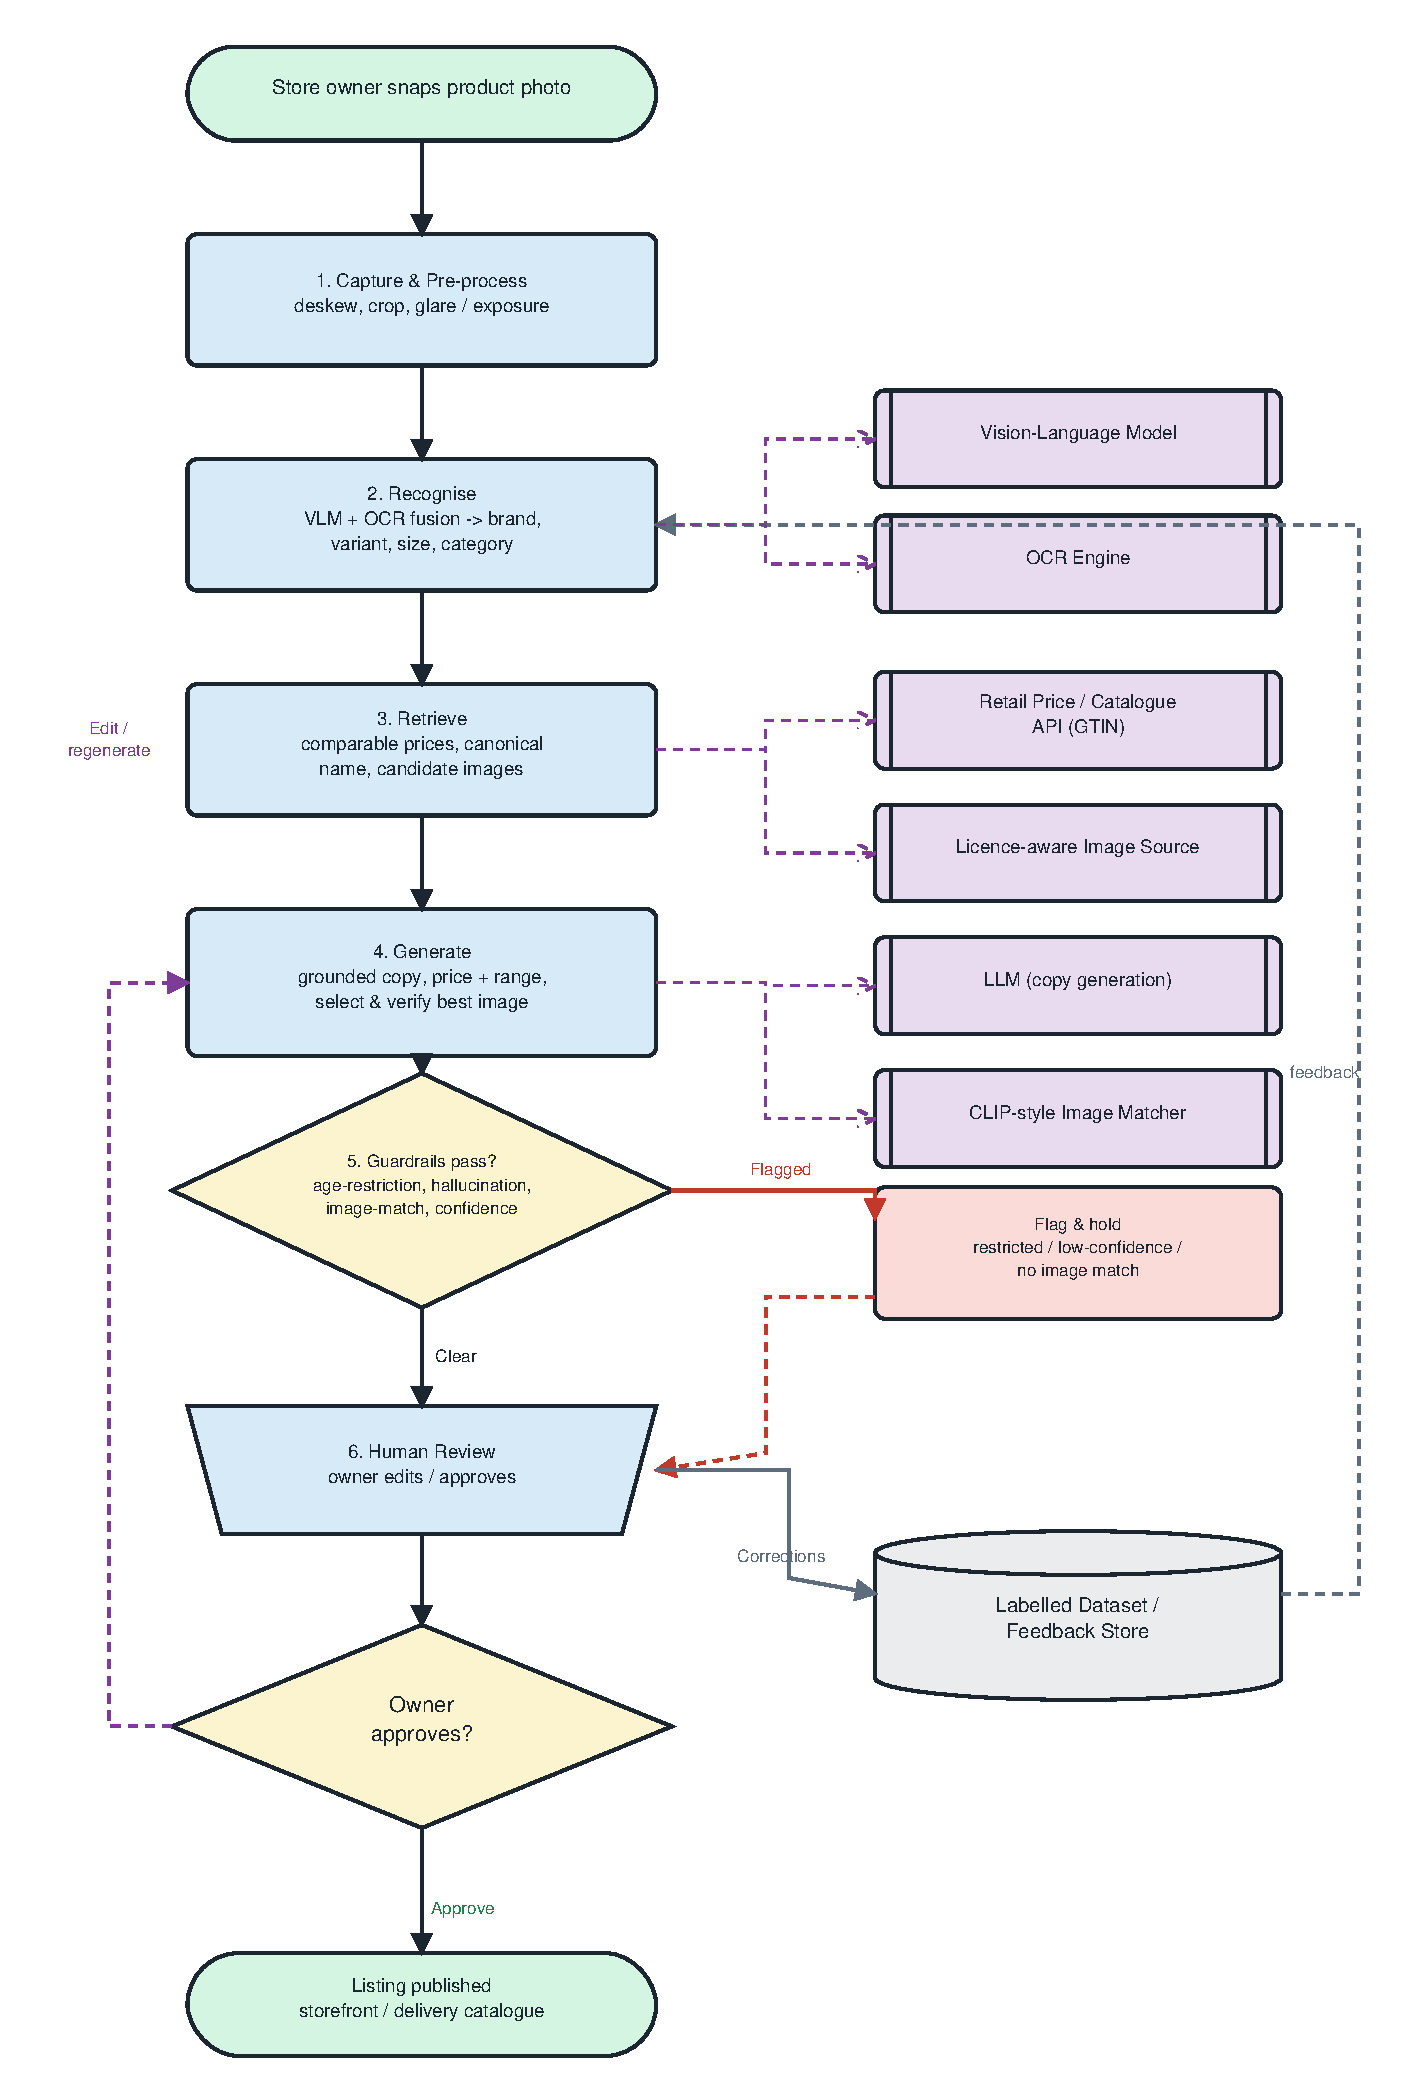
\includegraphics[width=\columnwidth]{architecture.pdf}}
\caption{End-to-end architecture: capture, recognise (VLM + OCR), retrieve (price, canonical
name, candidate images), generate, guardrails, human review, and publish, with a feedback loop
to a labelled store.}
\label{fig:arch}
\end{figure}

\begin{figure}[t]
\centerline{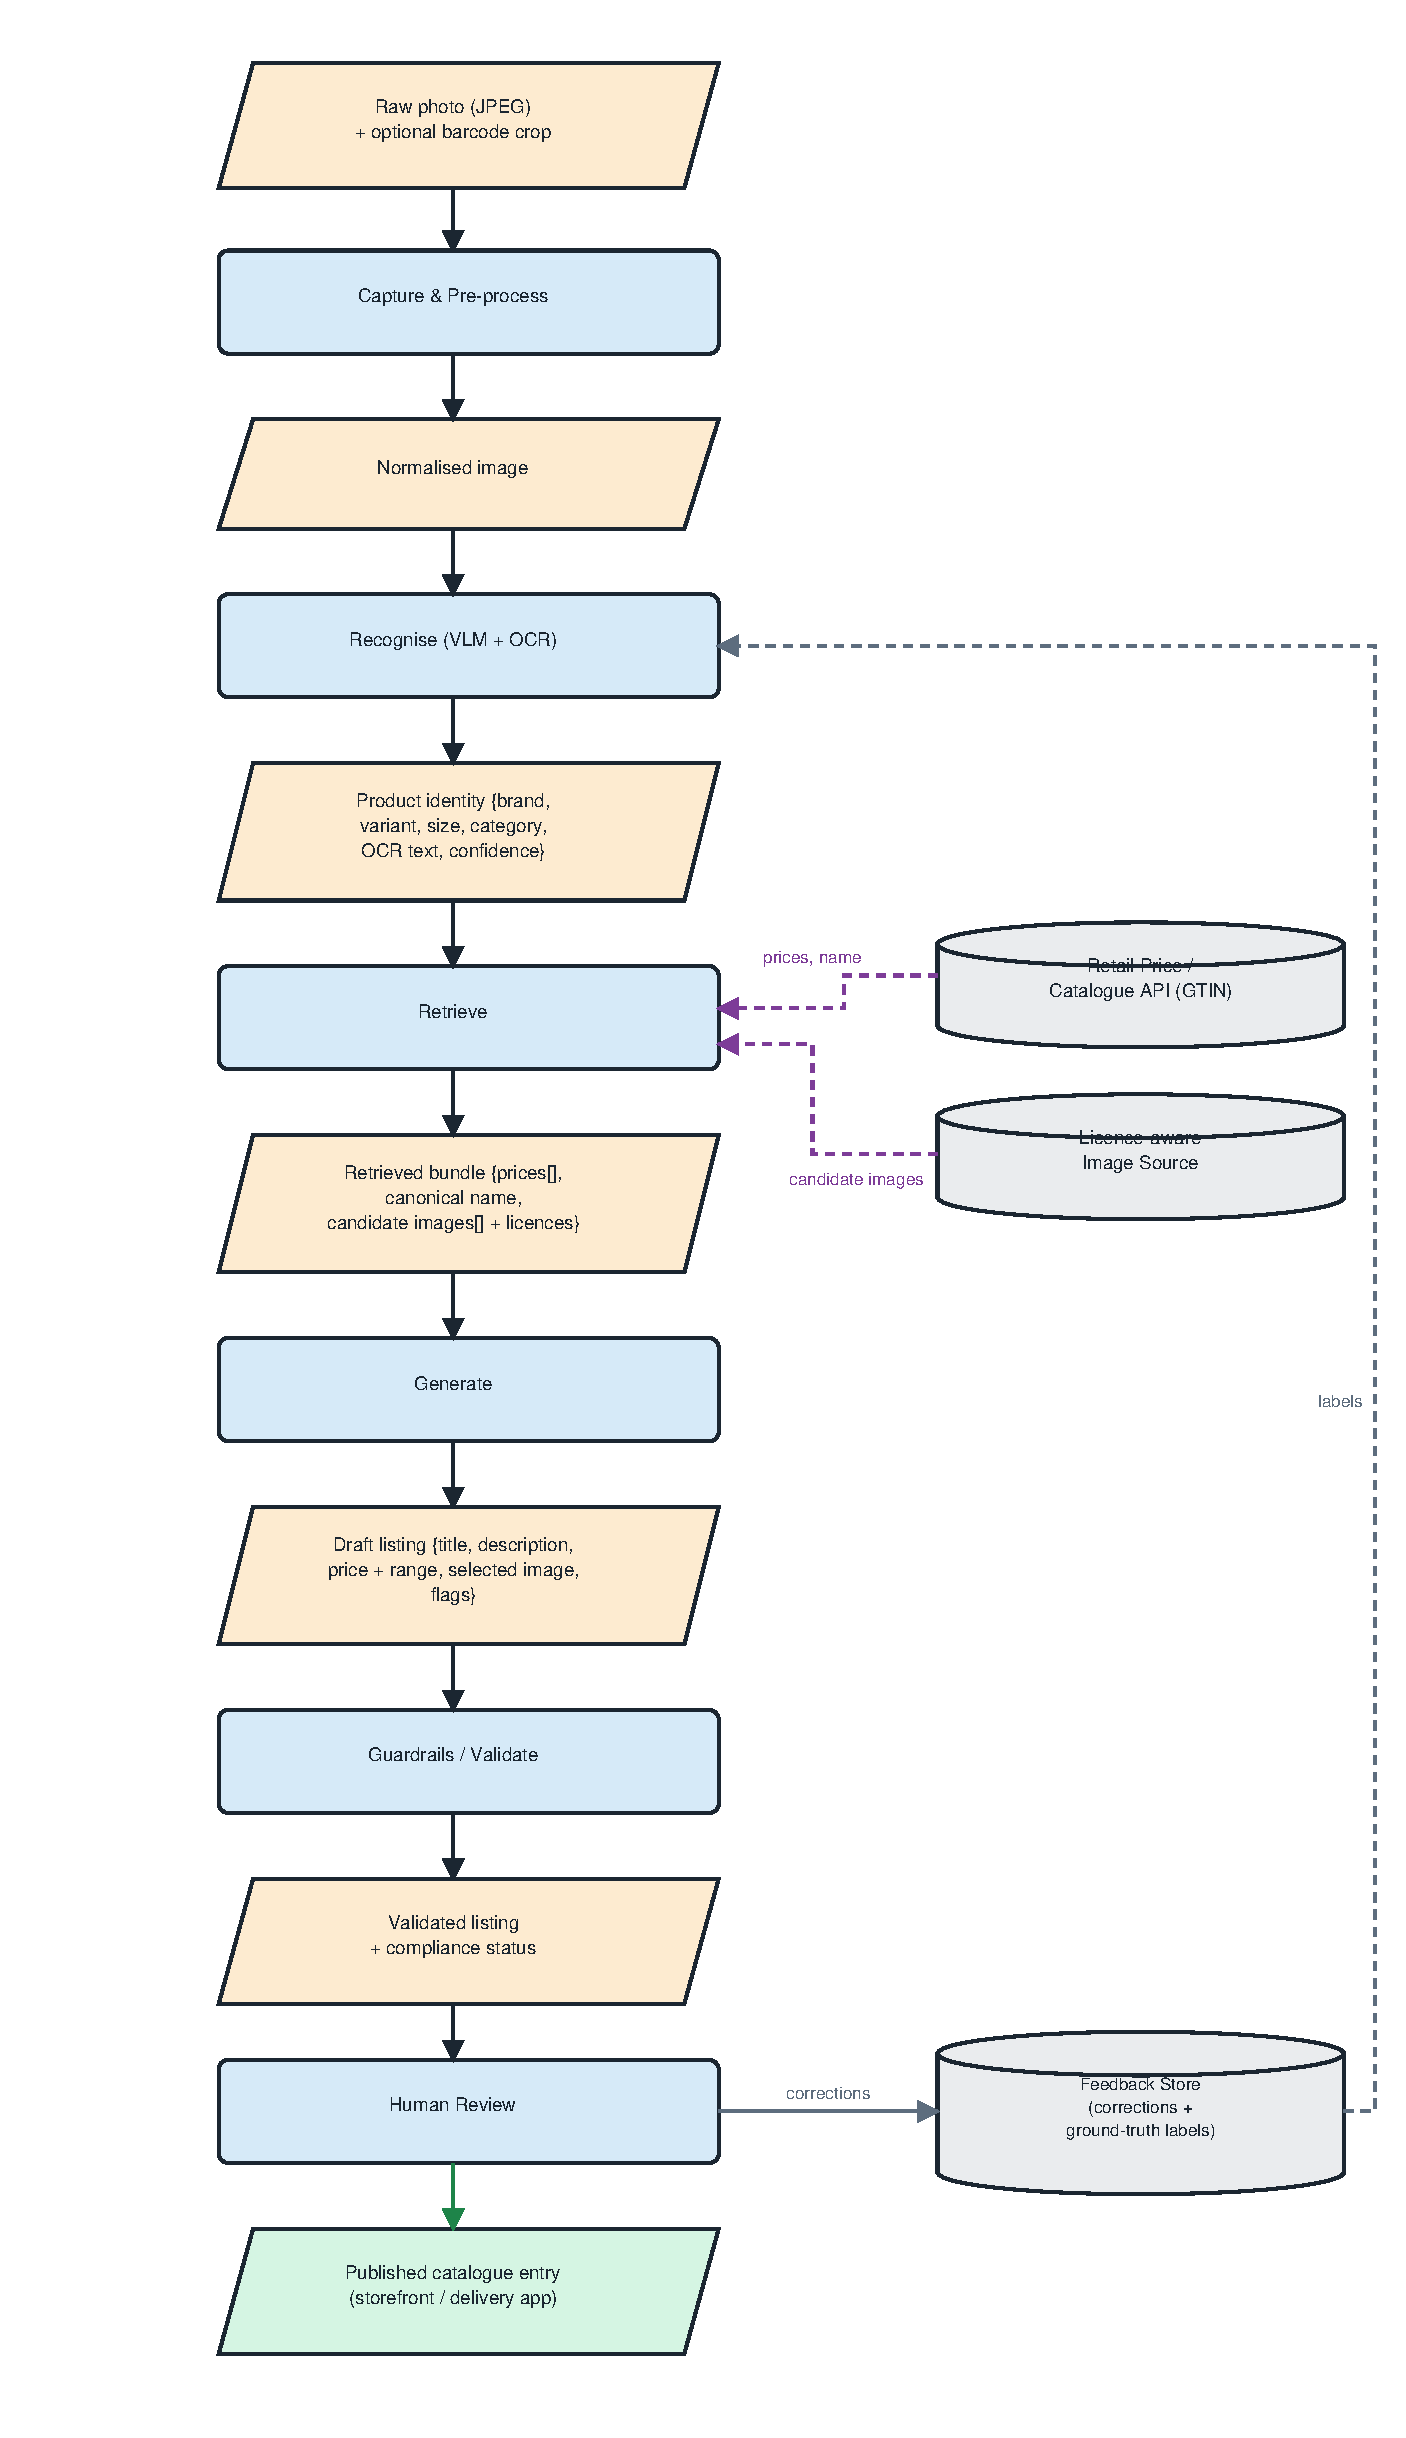
\includegraphics[width=\columnwidth]{dataflow.pdf}}
\caption{Data-flow view: the artifacts passed between stages, from raw photo to published
catalogue entry, with external datastores feeding retrieval.}
\label{fig:dataflow}
\end{figure}

%------------------------------------------------------------------------------
\section{Implementation and Design}
% TODO WS1/WS2/WS3/WS4: chosen models and architecture, data sources and preprocessing, the
% grounding and same-SKU image-match logic, confidence/guardrail thresholds, and the open-source
% stack (OpenCV; Qwen2-VL-2B/Moondream2 + PaddleOCR; Open Food Facts + Open Prices;
% Llama-3.2-3B/Qwen2.5-3B; OpenCLIP). Note zero training — all pretrained/zero-shot.

%------------------------------------------------------------------------------
\section{Results}
% TODO WS5: quantitative + qualitative results over the ~50-item test set vs the naive baseline.
% Populate Table~\ref{tab:results}. Add failure-mode discussion.

\begin{table}[t]
\caption{Pipeline performance on the [N]-item test set.}
\label{tab:results}
\centering
\begin{tabular}{@{}lcc@{}}
\toprule
Metric & Baseline & Snap-to-Sell \\
\midrule
Top-1 identification accuracy & TODO & TODO \\
Top-3 identification accuracy & TODO & TODO \\
Price median abs.\ \% error & TODO & TODO \\
Listing quality (blind rating) & TODO & TODO \\
Age-restriction recall & TODO & TODO \\
Image false-swap rate & TODO & TODO \\
\bottomrule
\end{tabular}
\end{table}

%------------------------------------------------------------------------------
\section{Conclusion and Future Work}
% TODO WS5: findings, objectives achieved, limitations (OFF coverage, small test set, no
% training), and future directions (fine-tuning, broader categories, live marketplace publishing).

%------------------------------------------------------------------------------
\section*{Acknowledgment}
% Optional. Note use of open datasets (Open Food Facts / Open Prices) and their licences.

%------------------------------------------------------------------------------
% While drafting, \nocite{*} lists every entry; remove once all real citations are in place.
\nocite{*}
\bibliographystyle{IEEEtran}
\bibliography{references}

\end{document}
